%\documentclass[aps,prl,reprint,superscriptaddress,nofootinbib]{revtex4-2}
\documentclass[aps,reprint,superscriptaddress,nofootinbib]{revtex4-2}

\usepackage[utf8]{inputenc}
\usepackage[english]{babel}
\usepackage{amsmath}
\usepackage{mathtools}
\usepackage{amsfonts}
\usepackage{csquotes}
\usepackage{bm}
\usepackage{indentfirst}
\usepackage{graphicx}
\usepackage{geometry}
\usepackage{minted}
\usepackage{hyperref}
\usepackage{subcaption}
\usepackage[font=small,labelfont=bf]{caption}
\usepackage{dcolumn}
\usepackage{tikz}
\usetikzlibrary{positioning}
\usepackage[noabbrev]{cleveref}
\usepackage{physics}
\usepackage{stmaryrd}
\usepackage{array}
\usepackage{cleveref}
\usepackage{multirow}
\usepackage{wrapfig}

\renewcommand{\arraystretch}{1.5}

\graphicspath{ {./figures/} }

\usepackage[T1]{fontenc}
\usepackage{mathptmx}

% This command exists in the physics package, and is hence ignored by the compiler. The physics package includes the functions
%       \norm{.} = ||.||, \abs{.} = |.|
%\newcommand{\norm}[1]{\left\lVert#1\right\rVert}

\begin{document}


%\title{Solving Differential Equations with Neural Networks and\\Grammar-based Genetic Algorithms: The Heat Equation}

\title{Finite differences, Neural Networks and Genetic Algorithms:\\The 3 Musketeers against the Heat equation} % apparently we're getting killed by Joao for this title :)






%%%%%%%%%%%%%%%%%%%
\author{J. G. Inácio}
\affiliation{Department of Physics, University of Oslo, Norway, Sem Sælands vei 24, 0371 Oslo}
%%%%%%%%%%%%%%%%%%%
\author{J. A. Fløisand}
\affiliation{Department of Physics, University of Oslo, Norway, Sem Sælands vei 24, 0371 Oslo}
%%%%%%%%%%%%%%%%%%%
\author{J. E. Kings}
\affiliation{Department of Physics, University of Oslo, Norway, Sem Sælands vei 24, 0371 Oslo}
%%%%%%%%%%%%%%%%%%%
\author{D. Aarstein}
\affiliation{Department of Physics, University of Oslo, Norway, Sem Sælands vei 24, 0371 Oslo}
%%%%%%%%%%%%%%%%%%%
\date{\today}
%%%%%%%%%%%%%%%%%%%
\begin{abstract}
    Genetic algorithms and neural networks are explored as possible ways to solve partial differential equations (PDEs) and ordinary differential equations (ODEs). First we implement the finite differences method to solve PDEs so we can have a baseline for comparison. We also implement a neural network using \textit{Tensorflow} capable of solving ODEs and PDEs. Lastly, we try to implement the method described in \cite{solving_diff_reproduce}, as well as make our own adjustments. The finite differences method proves reliable, albeit computationally burdensome due to the stability requirement. The neural network approach gives exceptionally good approximations in some cases. When it comes to the genetic algorithms we are in most cases able to reproduce the results from the original paper; for all ODEs and non-linear ODEs and three out of eight PDEs that we test, we find the analytical solution within the specified number of generations. Our own method finds the exact solution with a much greater success rate for all problems, but in general takes more generations than the original method for very simple problems.
    
    Our implementation can be found at \url{https://github.com/jgci2000/FYS-STK4155-projects}, under the \texttt{project\_3} (FDM and NN) and \texttt{project\_3\_genetic\_alg} (GA) folders.
\end{abstract}

\maketitle
%%%%%%%%%%%%%%%%%%%%%%%%%%%
%%%%%%%%%%%%%%%%%%%%%%%%%%%
\section{Introduction}
%%%%%%%%%%%%%%%%%%%%%%%%%%%
%%%%%%%%%%%%%%%%%%%%%%%%%%%

    Differential equations are the basis for our mathematical description of reality. In all sub-fields of physics, differential equations play a central role, as they often
    %, but not always,
    describe the way a system may evolve in time, given some conditions. % In between them,
    Among them, we find Newton's Second law, that tells us how the position of an object changes as we apply a force, or the famous Schrödinger equation, that tells us how a quantum state evolves in time, given its initial state. 
    Most often analytical solutions for these equations are difficult or impossible to attain. For example, Schrödinger's equation can only be solved analytically for a handful of problems, making numerical calculations a central aspect of getting predictions for difficult systems.
    
    Using some clever methods we can approximate their solution. The most known method is Euler's method, that stems %stands
    from the definition of the derivative.
    To solve more sophisticated problems, the finite differences method can be used.
    %To solve more sophisticated problems we are given the finite differences method.
    This method enables us to approximate first and second order derivatives through the truncation of the Taylor expansion of the given function. Although these methods are quite simple to understand and implement, they suffer from stability issues, making some problems impossible to solve.
    
    To avoid this stability problem, we can use neural networks to provide us the solution to some differential equations. This is possible due to the universal approximation theorem, which states that a neural network may approximate any function at a single hidden layer along with one input and output layer to any given precision. With some clever manipulation, we can use this fact to use neural networks to solve differential equations.
    
    These methods provide an approximation of the solution; however good that approximation is, there are situations in which we may want to obtain the exact closed-form analytical solution, if one exists. In this case, genetic algorithms, a process based on biological evolution and natural selection, can be used in combination with symbolic mathematics to deduce these analytical expressions rather flexibly.
    
    We will explore how the grammar-based genetic algorithm originally described by \cite{solving_diff_reproduce} can be leveraged and modified to reliably obtain analytical closed-form solutions to ODEs and PDEs alike.

    The aim of this work is to study the accuracy and advantages of using finite differences methods, neural networks and grammar-based genetic algorithms to numerically solve differential equations. In particular, we will study how these methods perform on the one-dimensional Heat equation.
    
    Our scripts and code authored for this project is all available at \url{https://github.com/jgci2000/FYS-STK4155-projects}, under the \texttt{project\_3} (FDM and NN) and \texttt{project\_3\_genetic\_alg} (GA) folders.

\section{Differential Equations}

    In general, a differential equation is an equation that contains some function \(f(\bm x):\mathbb{R}^n\to\mathbb{R}\) and its derivatives,
    \begin{equation*}
        g(\bm x, f(\bm x), \nabla f(\bm x), \nabla^2 f(\bm x), \ldots) = 0.
    \end{equation*}
    We can subdivide a differential equation into two sub-categories. A differential equation where \(f:\mathbb{R}\to\mathbb{R}\) is called an Ordinary Differential Equation (ODE), and only contains total derivatives of \(f\). %, since it can only contain total derivatives of \(f\). 
    A differential equation  where \(f:\mathbb{R}^n\to\mathbb{R}\), \(n > 1\), can contain partial derivatives, thus it is called a Partial Differential Equation (PDE).%The order of a differential equation is given by the highest order derivative present in the equation.
    
    The order \(n\) of an ODE, given by the highest order derivative present in the equation, will always give us \(n\) degrees of freedom through integration constants. We can therefore only hope to be able to find families of solutions. However, given initial conditions, we can find the exact solution, which provide additional information about the starting state of the system, or about what happens at the boundaries over time. For PDEs we have a similar phenomenon, but this time we can allow functions instead of constants. The initial conditions will be conditions on the function at the boundary of it's domain. 
    % To be able to solve these types of equations, we need some conditions. Such conditions gives us information about the solution at initial time or at the boundary of our problem. We can also have conditions that tell us how the derivative of the solution behaves at such points. Generally for a differential equation of order \(n\), we need \(n\) of those conditions.
    
\subsubsection{The Heat Equation} 
    
    The Heat Equation is a second order PDE that generally can be written as  
    \begin{equation} \label{eq:heat_general}
        \frac{\partial u}{\partial t} = \alpha \nabla^2 u,
    \end{equation}
    where \(\nabla^2:=(\frac{\partial^2}{\partial x_1^2},\ldots,\frac{\partial^2}{\partial x_m^2})^T\) is the Laplacian operator, \(\alpha \in \mathbb{R}\) and \(u = u(x_1, x_2, ... x_m, t)\), \(t>0\), is known as the temperature field. \(u\) tells us how the temperature in a space evolves over time, with the constant \(\alpha\) representing some properties of the physical system. 
    %This tells us how a given temperature field \(u\) evolves over time, with the constant \(\alpha\) representing some properties about the physical system. 
    
    We will in this report look at the one-dimensional case \(m=1\) with \(\alpha = 1\).
    % We will, however, restrict ourselves on the one-dimensional case \(m=1\), with \(\alpha = 1\). 
    This problem can be thought of as the time evolution of the temperature field of a rod of length \(L\) for an initial temperature field \(u(x, 0)\). 
    % \(x \in [0, L]\), given some initial temperature distribution \(u(x, 0)\). 
    The equation takes the form %as
    \begin{equation} \label{eq:heat}
        \frac{\partial u}{\partial t} = \frac{\partial^2 u}{\partial x^2}.
    \end{equation}
    In a more compact notation one can write \(u_t = u_{xx}\).
    We will consider the case \(L=1\) with boundary conditions % Thus our initial and boundary conditions are given as follows,
    \begin{align} 
        u(0, t) &= u(1, t) = 0; \\
        u(x, 0) &= \sin{(\pi x)}. \label{eq:custom_cond}
    \end{align}
    Physically, we will set the endpoints of the rod in a thermal bath at \(0K\) starting with a thermal field % distribution 
    on the rod given by \(\sin(\pi x)\). We expect the temperature to approach zero as time passes. When solving the equation numerically, we will restrict time to \(t\in[0,1]\). %
    %We would expect that, over time, the temperature would go to zero very quickly. So, we will also consider that \(t \in [0, 1]\).
    %
    % One can solve the equation by the separation of variables technique and find that the analytical solution is given by
    % \begin{equation} \label{eq:heat_anal}
    %     u(x, t) = \exp{(-\pi^2 t)} \sin{(\pi x)}.
    % \end{equation}
    \subsubsection{Solution to heat equation}
    Using separation of variables, i.e. assuming the solution is of the form \(u(x,t)=F(x)T(t)\), we find
    \begin{equation*}
        \frac{1}{T}\frac{dT}{dt}=\frac{1}{F}\frac{d^2F}{dx^2}
    \end{equation*}
    for equation \eqref{eq:heat}. We here assume that we are allowed to divide by \(F(x)\) and \(T(t)\) on both sides. As the left- and right hand sides only depends on time and position respectively, we are only left with the option
    \begin{equation*}
        \frac{1}{T}\frac{dT}{dt}=-k^2\quad\text{and}\quad\frac{1}{F}\frac{d^2F}{dx^2}=-k^2
    \end{equation*}
    for some \(k\in\mathbb{C}\). The solutions of these two equations are well known to be
    \begin{equation*}
        T(t)=e^{-k^2t}\quad\text{and}\quad F(x)=e^{ikx}.
    \end{equation*}
    We observe that \(u(x,t)=T(t)F(x)\) satisfies the differential equation \eqref{eq:heat}. By now using that $F(x) = e^{ikx} = a \cos(kx) + ib\sin(kx)$ and the first boundary condition, we have
    \begin{align*}
        u(0, t) &= 0\\
        e^{-k^2t}F(0) &= 0 \\
        e^{-k^2t}a &= 0 \\
        a = 0
    \end{align*}
    
    Using the other boundary condition we have
    \begin{align*}
        u(1, t) &= 0 \\
        e^{-k^2t}ib\sin(k) &= 0 \\
        \sin(k) &= 0
    \end{align*}
    which means that $k = n\pi$ for $n = 1, 2, \dots$
    
    Thus we have the solution as a linear combination of all the possible solutions given as
    \begin{equation*}
        u(x, t) = \sum_{n=1}^\infty c_n\sin(n\pi x)e^{-n^2\pi^2t}
    \end{equation*}
    
    Now using the initial condition we have that
    \begin{align*}
        u(x, 0) &= \sin(\pi x) \\
        \sum_{n=1}^\infty c_n\sin(n\pi x) &= \sin(\pi x)
    \end{align*}
    
    From which it is clear that only one coefficient contributes. That is $c_1 = 1$ and $c_n = 0$ for $n \geq 2$. Thus we have our final solution for $n=1$ and $k = n\pi = \pi$ given by
    \begin{equation} \label{eq:heat_anal}
        u(x,t)=e^{-\pi^2t}\sin(\pi x).
    \end{equation}
    
    % as \(u_k(x,t)=e^{ikx-k^2t}\).
    % %, and that \(u_k(x,t)=e^{ikx-k^2t}\) spans the solution space for \(k\in\mathbb{Z}\).
    % The solution \(u\) for the given boundary conditions will therefore be a linear combination of the different \(u_k\). The boundary condition \(u(0,t)=u(1,t)=0\) tells us
    % \begin{equation*}
    %     u(0,t)=\sum_{k\in\mathbb{Z}}\alpha_ke^{-k^2t}=\sum_{k\in\mathbb{Z}}\alpha_ke^{ik-k^2t}=u(1,t)=0.
    % \end{equation*}
    % Thus \(\alpha_0=0\) and \(\alpha_k=-\alpha_{-k}\) which means we are left with
    % \begin{equation*}
    %     u(x,t)=\sum_{k\in\mathbb{N}}2i\alpha_ke^{-k^2t}\sin(kx)=\sum_{k\in\mathbb{N}}\alpha_k^\prime e^{-k^2t}\sin(kx).
    % \end{equation*}
    % The initial condition \(u(x,0)=\sin(\pi x)\) then leaves us no other choice than choosing
    
%%%%%%%%%%%%%%%%%%%%%%%%%%%
%%%%%%%%%%%%%%%%%%%%%%%%%%%
\section{Methods}
%%%%%%%%%%%%%%%%%%%%%%%%%%%
%%%%%%%%%%%%%%%%%%%%%%%%%%%

    We will approach the problem in three different ways. First we will use the finite differences method to numerically solve the Heat Equation. Next we will construct a neural network code, using \textit{Tensorflow}, to solve both ODEs and PDEs and validate our implementation on some simple ODEs. Finally we will use a genetic algorithm that finds the solutions of differential equations as closed-form expressions.
    
    The absolute  error can be computed by evaluating
    \begin{equation*}
        \epsilon (x, t) = |u_e(x, t) - u(x, t)|
    \end{equation*}
    where \(u_e\) is the exact solution given by Equation \eqref{eq:heat_anal} and \(u\) is the solution by the numerical method. With genetic algorithms one should expect an error of zero, since the output is the analytical closed-form solution (for problems with a closed-form solution).

\subsection{Finite Differences}
    
    The finite differences method we will use in this report is based on the truncation of the Taylor expansion of a certain function to approximate the derivative at hand. 
    
    Let us consider a function \(f: \mathbb{R} \to \mathbb{R}\). Its Taylor expansion around a point \(x + h\) is given as
    \begin{align*}
        f(x + h) = f(x) + f^{'}(x) h + f^{''}(x) h^2 + ...
    \end{align*}
    Considering only the first order term, we get an approximation for the first derivative
    \begin{equation*}
        f^{'}(x) = \frac{f(x + h) - f(x)}{h}.
    \end{equation*}
    Considering a second order approximation and using the result above for the first derivative, we can get an approximation of the second derivative
    \begin{equation*}
        f^{''}(x) = \frac{f(x + h) - 2f(x) + f(x - h)}{h^2}.
    \end{equation*}
    
    By having an equispaced, discretized grid of \(N + 1\) points over \(x \in [0, X]\), \(x_0, x_1, x_2, \hdots, x_N\), given by
    \begin{equation*}
        x_i = i h = i \frac{X}{N},
    \end{equation*}
    \(i=0, \hdots, N\), we can write the above expressions as 
    \begin{align*}
        f^{'}(x) &\approx \frac{f(x_{i + 1}) - f(x_i)}{h} \\
        f^{''}(x) &\approx \frac{f(x_{i+1}) - 2f(x_i) + f(x_{i-1})}{h^2}.
    \end{align*}
    Thus, for the heat equation we have the following relation for \(u_t\) and \(u_{xx}\).
    \begin{align*}
        u_t &\approx \frac{u(x_j, t_{i + 1}) - u(x_j, t_i)}{\Delta t} \\
        u_{xx} &\approx \frac{u(x_{j+1}, t_i) - 2u(x_j, t_i) + u(x_{j-1}, t_i)}{(\Delta x)^2},
    \end{align*}
    where \(\Delta x\) and \(\Delta t\) are the distance between points in the equispaced grid of points, \(t_i = i\Delta t\), \(x_j = j\Delta x\). Applying these to the heat equation we get the following algorithm
    \begin{align*}
        u(x_j, t_{i + 1}) &= u(x_j, t_i) + \\\frac{\Delta t}{(\Delta x)^2} &(u(x_{j+1}, t_i) - 2u(x_j, t_i) + u(x_{j-1}, t_i)).
    \end{align*}
    
    Numerical methods for differential equations have a stability zone, where the method will converge to a stable solution. A discussion on stability and stability requirements is given by \cite{winther} and will not be presented in this report. We will, however, use the result that in order to achieve a stable solution it is necessary for the relation between $\Delta t$ and $\Delta x$ to satisfy the condition given by
    \begin{equation} \label{eq:stab}
        \frac{\Delta t}{(\Delta x)^2} < \frac{1}{2}.
    \end{equation}
    
    This means that if \(2\Delta t \geq (\Delta x)^2\) the method will never converge to a stable solution. In Figure \ref{fig:stab_reg} we can see the stability region for the given method. 
    \begin{figure}
        \centering
        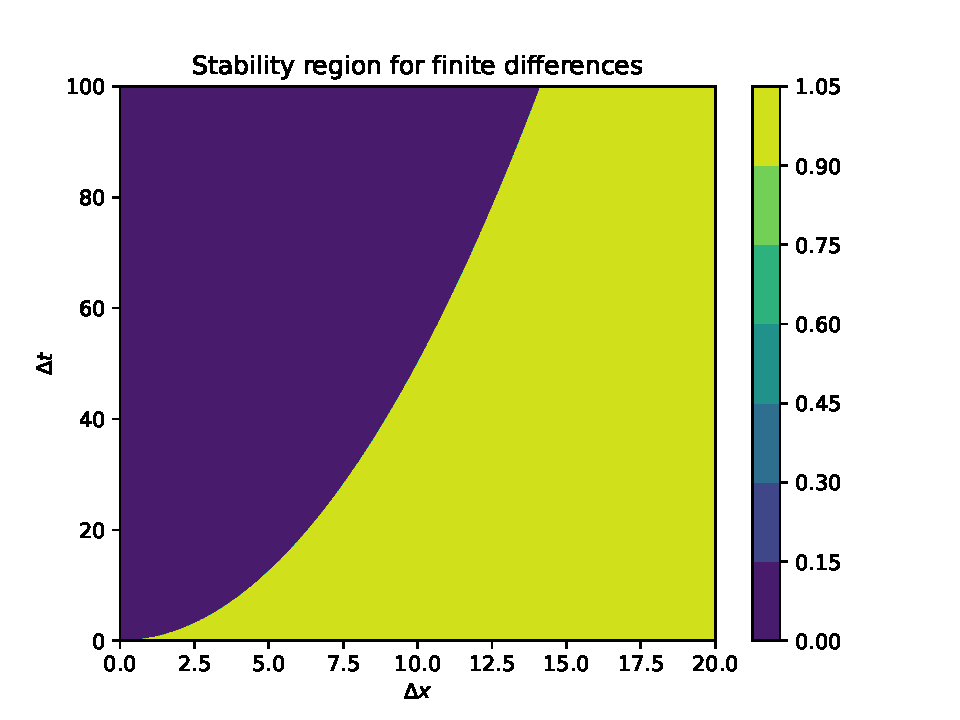
\includegraphics[scale=0.45]{figs/stability_region.pdf}
        \caption{Stability region for the finite differences method applied to the heat equation. Yellow indicates that the method will converge and blue indicates it will not converge with the selected values of \(\Delta x\) and \(\Delta t\).}
        \label{fig:stab_reg}
    \end{figure}
    
    With this method we are able to solve a plethora of systems. We just need to initialize our grid in such a way that it satisfies the given initial  conditions, as well as the stability requirement. We can thus solve problems where the temperature at the boundaries varies with respect to some non-differentiable function.
    
    The major problem as stated before is the stability condition, Equation \eqref{eq:stab}. This requires our time domain to be more discretized than our space domain. This makes our simulation much longer if we want a fine space domain.

\subsection{Neural Network for Differential Equations}

As in any other neural network, the cost function dictates the training of the network. Since we may write the differential equation in the form $g(\bm x, f(\bm x), \nabla f(\bm x), \nabla^2f(\bm x), \dots) = 0$, we may then choose $C(\bm x, P) = g^2$ to be the cost functions which we intend to minimize. Here $\bm x$ is the vector which contain parameters for the problem, and $P$ is the parameters of the network, i.e. the weights and biases.

The neural network approach works by having a trial solution which is dependent on the initial conditions, boundary conditions and a neural network. This is achievable by letting the trial solution be a sum of functions, where some ensure the conditions and some use the neural network in order to make the trial function as close as possible to the true solution. 

The trial solution is initialized with random weight and biases, and by using high precision numerical differentiation the gradient of the cost function can be calculated with respect to $P$. For each epoch the gradient is calculated and the weights and biases appropriately updated. For this project the learning rate was chosen to be constant but this is not a necessity.

After sufficiently many epochs the trial solution should have minimized the cost function, and has hence given us the approximation of the true solution. A prediction can then be made by having the parameters of $\bm x$ as nodes in the input layer. The network should return one value which is the predicted value of the true solution for the given input.

\subsubsection{Implementation}

In the case of the one-dimensional heat equation we may write our trial solution as
\begin{equation*}
    S(x, t, NN(x, t; P)) = h_1(x) + h_2(x, t, NN(x, t; P))
\end{equation*}
with
\begin{equation*}
    h_1(x) = \sin(\pi x)
\end{equation*}
and
\begin{equation*}
    h_2(x, t, NN(x, t; P)) = x(1-x)t \cdot NN(x, t; P)
\end{equation*}
Note that $S$ satisfies the initial- and boundary conditions. This is because
\begin{align*}
    S(0, t, NN) &= \sin(\pi \cdot 0) + 0 \cdot t\cdot NN(0, t; P) = 0 \\
    S(1, t, NN) &= \sin(\pi) + 1\cdot 0 \cdot t \cdot NN(1, t; P) = 0
\end{align*}
as given by $u(0, t) = u(1, t) = 0$, and
\begin{align*}
    S(x, 0, NN) &= \sin(\pi x) + x(1-x) \cdot 0 \cdot NN(x, 0; P) \\
    &= \sin(\pi x)
\end{align*}
as given by $u(x, 0) = \sin(\pi x)$. \\
This construction also ensures that the trial solution $S$ is differentiable with respect to time, and twice differentiable with respect to the position, a property which is found in the true solution.

In this project \textit{Tensorflow} was leveraged %implemented
in order to create the neural network. This also allowed for finding the gradient of the cost function with respect to the parameters of the neural network, due to under-the-hood properties of the package.
Using the neural network method for solving other differential equations works in a similar manner: we find the appropriate functions \(h_i\) which comprise \(S\) and use them to minimize the cost function.%Find the appropriate functions $h_i$ which comprise $S$ and minimize the cost function.

%Our network was initiated with (this changes? So perhaps it should be in results)
% gj daniel :) 8====D~~~~~

\subsubsection{Benefits and Shortcomings}

% daniel spiser fitta, fitte** 8==D~~~(.Y.) 38008 _____
The strength of this way of approximating a differential equation lies in its ability to train itself to a sufficient accuracy with very limited data, namely the grid of combinations (inputs) and the target that every point should be zero. Simply by calculating the loss with the cost function, the model updates itself for the desired amount of epochs.

Another benefit is that it translates very well to problems of higher dimensionality. With traditional methods, going from a 2-dimensional problem to a 3-dimensional problem increases the computational load by one order of magnitude. With the neural network approach it might not be necessary to change the number of epochs or layer design at all. This, however, is very unlikely, some changes might be needed in order to ensure that the approximation is as good as possible.

These benefits do not come without some inconveniences though. 
In contrast with the finite differences method, the neural network does not allow for hard-coded boundary values. This is a result of the underlying difference between the two methods. The finite differences method calculates the next value based on its surroundings, the neural network tries to guess the underlying function which would solve the problem as a whole. Therefore the boundary conditions and initial conditions needs to be contained in the trial solution, as it would have been in the true, analytical solution. This does restrict the complexity of our conditions.

For instance, solving the heat equation of a one dimensional rod with $u(1, 0) = T$ and $u(1, t) = 0 \; \text{for} \; t > 0$ is not possible, due to the discontinuous nature of the temperature applied to the end of the rod.

Additionally, the initial and boundary conditions decide the properties of the functions which comprise $S$, i.e. $h_1, h_2, \dots, h_n$. With complicated conditions finding appropriate $h_i$ functions might prove to be quite troublesome.

% Nonetheless, boundary conditions can be used, we only had success with the conditions being described by continuous functions.
Boundary conditions can be used, but we only had success with conditions described by continuous functions in our trials.

Another shortcoming is that the neural network model does not allow for Neumann boundary conditions. That is, we may not have conditions on the derivatives of the trial solution.
As an example; the ODE $y'' + y = 0 \; \text{for} \; y \in [a, b]$ with the conditions $y'(a) = \alpha, y'(b) = \beta$ is not solvable with this approach. This is due to the structure of our trial solution, which contains the network, which in turn depends on the parameters of our equation $\bm x = [x, t, etc.]$. Due to the chain rule the term $\pdv{NN}{\bm x}$ will appear, and due to the network changing for each epoch, its impossible to control $\pdv{NN}{\bm x}$ such that $\pdv{S(\bm x, NN(\bm x))}{\bm x} = f(\bm x)$ for any $f(\bm x)$. This holds true even for simple cases, for instance $f(\bm x) = \alpha$ for some constant $\alpha \in \mathbb{R}$.


\subsection{Genetic Algorithm for Differential Equations}

\subsubsection{Genetic Algorithms}

Much like neural networks, genetic algorithms are a learning method based at the outset on a biological process. However, unlike NNs, genetic algorithms are by nature much more akin to a directed random walk influenced by processes inspired by evolution and natural selection, and do not require gradient descent methods, which can make them much more flexible to solve problems where gradient descent isn't necessarily applicable, \cite{gen_book}.

The basic premise of genetic algorithms is the initialization of a population of individuals, or agents, of size \(N\), each corresponding to a potential, randomly selected solution to the problem at hand. Each of these agents can be seen as a haploid organism (single chromosome) with gene vector \(\Gamma\) of size \(n\), \(\Gamma = \left(\gamma_0, \gamma_1, \ldots, \gamma_{n-1}\right)\). Typically, the domain in which individual genes \(\gamma_i\) are defined is chosen depending on what is being modelled, \cite{parameterless_ga}, and can be \(\mathbb{B} = \{0, 1\}\), \(\mathbb{N}\), \(\mathbb{R}\), etc; here, we shall use the notation \(\Gamma \in \mathbb{G}^n\) to encompass the relevant domain in a general way. The genes must follow the requirement of being deterministically decodable into the potential solution proposed by the individual following a \textit{grammar} \(\Sigma\left(\Gamma\right): \mathbb{G}^n \to \mathbb{S}\) which can be thought of as the conversion step from the individual's genetic composition (its \textit{genotype}) to the actual observable characteristics obtained by expression of the genes (the individual's \textit{phenotype}). \(\mathbb{S}\) here denotes the solution space.

A given problem is modelled by a fitness function \(\Phi: \mathbb{S} \to \mathbb{R}^+\), comparable to a cost function, \cite{ga}, that we want to minimize. Hence, given an individual \(\Gamma^{(i)} \in \mathbb{G}^n\), its fitness value is given by
\begin{align*}
    \phi^{(i)} &= \Phi\left(\Sigma\left(\Gamma^{(i)}\right)\right)
\end{align*}

The goal of genetic algorithms is to model the process of natural selection. In order to achieve this, at each iteration, or \textit{generation}, the fitness \(\phi\) of each individual is computed in order to sort the population. Based on this metric and a set replication rate \(r \in [0,1]\), the \(\lfloor(1-r)N\rfloor\) lower scoring agents are removed from the pool. To replace them, a set of genetic operators \(\alpha(\Gamma) = \Gamma^{~\prime}\) are applied to the top \(\lceil rN\rceil\) agents. These genetic operators attempt to model the process of reproduction in real-life, wherein organisms give birth to children similar genetically, but with slight differences (or \textit{mutations}) that may or may not give a random advantage to the child. The key is that these operations do not inherently need to benefit child individuals; a purely random modification of the genotype will most likely create a new phenotype, which could benefit the individual and give birth to new characteristics that advance the population as a whole towards the solution(s) of the problem at hand in the next generations, \cite{genotype_phenotype}.

There are many different types of genetic operators, such as BSP-based solutions to eliminate genetic clones, \cite{non_revisiting_ga}, or crossover and mutation variants, \cite{ga}, but the main ones are the \textit{crossover}, in which two parent agents with chromosomes \(\Gamma^{(a)}\) and \(\Gamma^{(b)}\) are selected among the fittest in the population, to give birth to two children \(\Gamma^{(a)\prime}\) and \(\Gamma^{(b)\prime}\) by the random selection of a value \(m \in [1, n-2]\), where \(\Gamma^{(a)\prime}\) inherits the genes \([0,m-1]\) from \(\Gamma^{(a)}\) and the genes \([m,n-1]\) from \(\Gamma^{(b)}\), and inversely for \(\Gamma^{(b)\prime}\):
\begin{align*}
    \Gamma^{(a)\prime} &= \left(\gamma_0^{(a)}, \ldots, \gamma_{m-1}^{(a)}, \gamma_{m}^{(b)}, \ldots, \gamma_{n-1}^{(b)}\right)
    \\
    \Gamma^{(b)\prime} &= \left(\gamma_0^{(b)}, \ldots, \gamma_{m-1}^{(b)}, \gamma_{m}^{(a)}, \ldots, \gamma_{n-1}^{(a)}\right)
\end{align*}

Another popular genetic operator is a simple mutation, in which each chromosome \(\Gamma^{(i)}\) selected for mutation (typically, this can be all of the children created at the end of the generation) is associated a random value \(m^{(i)} \in [0, n-1]\) and is then modified to become
\begin{align*}
    \Gamma^{(i)\prime} &= \left(\gamma_0^{(i)}, \ldots, \gamma_m^{(i)\prime}, \ldots, \gamma_{n-1}^{(i)}\right)
\end{align*}
where \(\gamma_m^{(i)\prime}\) is a randomly selected value from \(\mathbb{G}\). Note that \(\gamma_m^{(i)\prime}\) may or may not depend on the value of \(\gamma_m^{(i)}\) depending on the implementation, \cite{ga}, for example by a simple displacement by \(\delta\gamma\) following a Gaussian distribution (applicable only in the case \(\mathbb{G} = \mathbb{R}\)), or by flipping the bit \(\gamma_m^{(i)}\) (applicable if \(\mathbb{G} = \mathbb{B}\)).

\subsubsection{Original Method}

In order to solve ODEs and PDEs with genetic algorithms, we follow very closely the method introduced and discussed by Tsoulos and Lagaris in \cite{solving_diff_reproduce}. There are two main ingredients that make this method special: the grammar \(\Sigma\) and the fitness function \(\Phi\).

% How the grammar is set up
To produce closed form analytical solutions to ODEs and PDEs, \(\Sigma\) must be set up to decode chromosomes (defined here on \(\mathbb{G}^n = \mathbb{N}_0^n\)) into symbolic mathematical expressions. To do so, we define 4 types of sub-expressions: functions \(f\), operations \(o\), constants \(c\) and variables \(v\), as:
% \begin{align*}
%     &\Sigma \Coloneqq
%     \\
%     &f: \left\{\sin(\sigma),~\cos(\sigma),~\exp(\sigma),~\ln(\sigma)\right\},
%     \\
%     &o: \left\{\left(\sigma_1+\sigma_2\right),~\left(\sigma_1-\sigma_2\right),~\left(\sigma_1\times\sigma_2\right),~\frac{\sigma_1}{\sigma_2},~\sigma_1^{\sigma_2}\right\}
%     \\
%     &c: \mathbb{R}
%     \\
%     &v: \left\{x, y\right\}\text{\footnotemark}
% \end{align*}
\begin{align*}
    &f\in \left\{\sin(\sigma),~\cos(\sigma),~\exp(\sigma),~\ln(\sigma)\right\},
    \\
    &o\in \left\{\left(\sigma_1+\sigma_2\right),~\left(\sigma_1-\sigma_2\right),~\left(\sigma_1\times\sigma_2\right),~\frac{\sigma_1}{\sigma_2},~\sigma_1^{\sigma_2}\right\}
    \\
    &c\in \llbracket0,9\rrbracket := \{0,1,\ldots,9\} %[0,9]
    \\
    &v\in \left\{x, y\right\}\text{\footnotemark}
\end{align*}
\addtocounter{footnote}{-1}
\footnotetext{Note that the subset \(v\) depends on the dimensionality of the problem we're trying to solve; for ODE problems, we take instead \(v: \left\{x\right\}\); for three-dimensional PDE problems, we take \(v: \left\{x, y, z\right\}\); and so on. Here, we focus on two-dimensional PDEs, since that's the form the 1D heat equation takes.}
where \(\sigma, \sigma_1, \sigma_2\) denote instances of sub-expressions.
%An entire expression can be built by selecting one of the four groups, selecting one of the group's members, and recursively replacing the \(\sigma\)s with sub-expressions selected again from \(f\), \(o\), \(c\) and \(v\) themselves.
Expressions are built by selecting one of the four groups, then selecting an element from this group, and recursively replacing sub-expressions \(\sigma\) within this element with sub-expressions selected again from \(f\), \(o\), \(c\) and \(v\).
It should be noted that there are slight differences between our version of this grammar and the original from \cite{solving_diff_reproduce}; in particular, we add \(\sigma_1^{\sigma_2}\) to the list of available operations.

This restricted grammar has a few advantages over trying to generalise to fit every possible mathematical expression. It can represent a wide variety of closed-form expressions (and can easily be extended to cover more functions, operations, etc), and it is trivial to compute the symbolic derivatives of these expressions by recursively applying well-known differentiation rules to the individual sub-expressions\footnote{Note that, to keep the implementation simple, the power operation \(\sigma_1^{\sigma_2}\) is limited to constant expressions for \(\sigma_2\) in order to compute the derivatives efficiently -- as such, the expressions \(x^2\), \(y^{\cos(\pi + 3)}\) and \(\ln(x)^{\exp(5)}\) are allowed, but not \(5^x\).}. It is also trivial to convert a chromosome \(\Gamma\) into an expression; each gene is looked at sequentially, representing an index into the superset \(\left\{f, o, c, v\right\}\) or one of its individual sets, building up the entire symbolic expression recursively. For example, the chromosome \(\Gamma = \left(0, 0, 1, 2, 2, 5, 3, 0, \ldots\right)\)\footnote{The actual length of the chromosome doesn't matter much, as long as it is long enough to encode the full expression; genes beyond the point where a valid expression has been decoded are simply ignored. If it is not, \cite{solving_diff_reproduce} recommend allowing up to 2 wraparounds, where \(\gamma_n = \gamma_0, \gamma_{n+1} = \gamma_1, \gamma_{2n+3} = \gamma_3\), etc. If the expression is still not complete, it can be marked as invalid and discarded by being given a fitness value of \(+\infty\). In our implementation, we choose to mark the expression as invalid immediately instead of allowing any wraparounds, as a gene with alleles that encode two or more completely separate parts of the final expression will have a very hard time mutating and remaining coherent through generations regardless.} can be decoded into the expression \(\sin(5x)\), Table \ref{tab:expr_example}.

Note that, when selecting elements from these limited sets, the modulo operator is used on the gene value with regards to the size of the sampled set; i.e., if \(\gamma_i = 17\) and locus \(i\) represents, in context, a function out of \(f\), the decoded value is \(\sigma = f_{\gamma_i \mod 4} = f_1 = \cos(\ldots)\).

\begin{table}[htp]
    \centering
    \caption{Decoding of the example expression \(\sin(5x)\) built up from a chromosome \(\Gamma = \left(0, 0, 1, 2, 2, 5, 3, 0, \ldots\right)\) through \(\Sigma\).}
    \begin{tabular}{c|c|c|c}
        \(\gamma_i\) & Contextual meaning & Target & Expression
        \\
        \hline 
        0 & \(\Sigma(0) = f\) & \(\sigma_0\) & \(func(\sigma_1)\)
        \\
        0 & \(f_0 = \sin(\sigma)\) & \(func\) & \(\sin(\sigma_1)\)
        \\
        1 & \(\Sigma(1) = o\) & \(\sigma_1\) & \(\sin(op(\sigma_2, \sigma_3))\)
        \\
        2 & \(o_2 = \sigma \times \sigma\) & \(op\) & \(\sin(\sigma_2 \times \sigma_3)\)
        \\
        2 & \(\Sigma(2) = c\) & \(\sigma_2\) & \(\sin(const \times \sigma_3)\)
        \\
        5 & \(c_5 = 5\) & \(const\) & \(\sin(5 \times \sigma_3)\)
        \\
        3 & \(\Sigma(3) = v\) & \(\sigma_3\) & \(\sin(5 \times var)\)
        \\
        0 & \(v_0 = x\) & \(var\) & \(\sin(5 \times x)\)
    \end{tabular}
    \label{tab:expr_example}
\end{table}

The expressions generated by the grammar can also be thought of as binary trees, where the root node is the whole expression, the leaf nodes are the dimensional variables \(v\) and constants \(c\), and intermediate nodes represent functions (with one child node) and operations (two child nodes). As an example, consider the function \(f(x, y) = \ln(x)\exp(3y+x)\); one possible expression tree that represents this function that abides to \(\Sigma\) is shown in Figure \ref{fig:expr_tree}. Note that this is just one of many possible representations of this expression (such as \(1\times\exp(-2x+3(x+y))\ln(x+0)\) for example), and in fact there are infinitely many trees that represent the same function. This means that an infinite amount of chromosomes \(\Gamma\) can express the exact same phenotype, which is something we shall try to mitigate later on in order to optimize the evolution towards one solution.

\begin{figure}[htp]
    \centering
    \includegraphics[width=0.5\linewidth]{figs/genetic_diagrams/expr_tree.png}
    \caption{Expression tree representing \(\ln(x)\exp(3y+x)\)}
    \label{fig:expr_tree}
\end{figure}

% How the fitness function is set up
On top of the definition of the grammar, a fitness function \(\Phi\) must be set up to take any ODE or PDE on a defined domain, mapping the encoded expressions \(\sigma\) into positive fitness values corresponding to how close or far an expression is from the analytical solution; \(\Phi(\sigma) \in \mathbb{R}^+\). We introduce here the fitness function initially set up by \cite{solving_diff_reproduce}.

Let \(D\subseteq\mathbb{R}^d\) be the domain of our differential equation\footnote{Here \(H_f(\bm{x})\) denotes the Hessian of \(f\) evaluated at \(\bm{x}\). The \(\ldots\) is meant to include all other partial derivatives \(\frac{\partial^k f}{\partial x_1^{i_1}\ldots\partial x_d^{i_d}}\) as long as they exist. (Here \(\sum_{n=1}^di_n=k\).)} \(g\left(\bm x, f(\bm x), \nabla f(\bm x), H_f(\bm x), \ldots\right) = 0\), i.e., \(f:D\to\mathbb{R}\). Let \(\partial D_i\) denote one boundary of the domain \(D\) and assume we are given some boundary conditions \(g_i:\partial D_i\to\mathbb{R}\), \(g_i\left(\bm x, f(\bm x), \nabla f(\bm x), H_f(\bm x), \ldots\right) = 0\). To get an expression for the fitness, we divide our domain into a set of discrete, linearly spaced points denoted \(\widetilde{D}\). The set of points on boundary \(i\) will be denoted by \(\partial\widetilde{D}_i\). We define the fitness of an encoded expression \(\sigma\) as
\begin{align*}
    \Phi(\sigma) = &\sum_{\bm{x}\in\widetilde{D}}g\left(\bm{x}, \sigma(\bm{x}), \nabla\sigma(\bm{x}), \ldots\right)^2 + 
    \\
    &\lambda\sum_i\sum_{\bm{x}\in\partial\widetilde{D}_i}g_i\left(\bm{x}, \sigma(\bm{x}), \nabla\sigma(\bm{x}), \ldots\right)^2,
\end{align*}
where \(\lambda\) is a penalty regularization parameter for the boundary conditions. For ODEs we will generally choose \(\widetilde{D}\) as 10 values of \(x\), and for two-dimensional PDEs we generally choose \(50\times50\) discrete points \((x, y)\). We will also generally put the penalty \(\lambda\) to 100.

An advantage of computing the fitness this way over the neural network method is that it supports arbitrary boundary conditions, including Neumann boundary conditions, rather than simply Dirichlet boundary conditions. It is also highly generalizable to non-linear differential equations and can be easily applied in arbitrarily high dimensions.

% Maybe i'll add an example ODE & expression to show how the fitness value is computed here
As an example, consider the ODE
\begin{align*}
    g(x) = \frac{d^2}{dx^2}f(x) + 100\frac{d}{dx}f(x) &= 0
\end{align*}
defined on \([0, 1]\) with boundary conditions
\begin{align*}
    g_0(x) = f(0) &= 0
    \\
    g_1(x) = \frac{d}{dx}f(0) - 10 &= 0
\end{align*}
This ODE has analytical solution \(f(x) = \sin(10x)\). Taking an example decoded expression
\begin{align*}
    \sigma(x) = e^{-x}-1,
\end{align*}
the fitness of \(\sigma\) with respect to \(g, g_1, g_2\) is given by
\begin{align*}
    \Phi(\sigma) =& \sum_{x\in\widetilde{D}}g\left(x, \sigma(x), \frac{d}{dx}\sigma(x), \frac{d^2}{dx^2}\sigma(x)\right)^2 + 
    \\
    &\lambda\sum_{i=0}^1\sum_{x\in\partial\widetilde{D}_i}g_i\left(x, \sigma(x), \frac{d}{dx}\sigma(x)\right)^2
    \\
    \Phi(\sigma) =& \sum_{x\in\widetilde{D}}\left(\frac{d^2}{dx^2}\sigma(x) + 100\frac{d}{dx}\sigma(x)\right)^2 +
    \\
    &\lambda\sum_{x\in\partial\widetilde{D}_0}\sigma(x)^2 + \lambda\sum_{x\in\partial\widetilde{D}_1}\left(\frac{d}{dx}\sigma(x)-10\right)^2
\end{align*}
where \(\frac{d}{dx}\sigma(x) = -e^{-x}\) and \(\frac{d^2}{dx^2}\sigma(x) = e^{-x}\). We have \(\partial\widetilde{D}_i = \{0\}\) for both boundary conditions, and, taking \(\widetilde{D} = \{0, 0.25, 0.5, 0.75, 1\}\) and \(\lambda = 100\), this yields a fitness of
\begin{align*}
    \Phi(\sigma) =& \sum_{i=0}^4 \left(- 99e^{-\frac{i}{4}} + 99\right)^2 +
    \\
    &100 \left(e^0-1\right)^2 + 100\left(-e^0-10\right)^2
    \\
    \Phi(\sigma) \approx& 2 \times 10^4
\end{align*}
This is a really high fitness score, indeed indicating that \(\sigma(x) = e^{-x}-1\) is not a very good fit to the ODE here.

One thing to note is that the original method proposed by \cite{solving_diff_reproduce} is also applicable to systems of ODEs with a modification on the interpretation of chromosomes by the grammar and on the fitness function. Since the focus here is ODEs and PDEs, we will not delve into how this is set up and do not implement this variation.

\subsubsection{Our Method}

Having implemented and tested the original method from \cite{solving_diff_reproduce}, we feel that it is lacking in some aspects, and is prone to failing on problems with more difficult analytical expressions. We have already discussed a few modifications made to the original method (such as allowing for power operations), but the main drawback we see is the way expressions are inferred from chromosomes.

% Discuss why their chromosomes make no sense
The way chromosomes are decoded into expressions is sequential. Hence, the meaning of each allele \(\gamma_{i+1}\) is very highly dependent upon the value \(\gamma_{i}\). Taking the example chromosome from earlier, \(\Gamma = \left(0, 0, 1, 2, 2, 5, 3, 0, \ldots\right)\) and changing the third gene from \(\gamma_2 = 1\) to \(\gamma_2 = 0\), the decoded expression becomes \(f(x) = \sin(\exp(5)) \approx -0.7\) instead of \(f(x) = \sin(5x)\). As another example, changing the first gene from \(\gamma_0 = 0\) to \(\gamma_0 = 3\), the expression goes from \(f(x) = \sin(5x)\) to \(f(x) = x\).

These disparities happen because a linear sequence is being decoded into a tree, which has a higher dimensionality, and therefore small modifications and mutations in the original sequence will have drastic effects on the structure of the expression tree itself. In practice, this means that, given an individual \(\Gamma\) with very low fitness, there is no guarantee whatsoever that a descendent \(\Gamma^{~\prime}\) (highly similar to \(\Gamma\) genetically) will share any resemblance phenotypically. Therefore, it is very likely that, in the event that \(\Gamma^{~\prime}\) has a lower fitness score than \(\Gamma\), it is by a product of purely random chance more than natural selection. Or, considering agents as being assigned points on the multi-dimensional surface representing their fitness, an agent's descendents can suddenly jump extremely far from where their parent stands from one generation to the next, thus discouraging steady evolution towards the final solution. Ideally, we want agents to evolve slowly towards the solution with small, incremental changes, such as modifying \(f(x) = \sin(5x)\) into \(f(x) = \sin(4.8x)\) or into \(f(x) = \cos(5x)\)\footnote{Arguably, going from \(\sin(5x)\) to \(\cos(5x)\) is already a large jump and will likely result in a great increase or decrease in fitness; however, measured jumps are necessary to arrive at the solution eventually, and are at the core of genetic algorithms. What we try to prevent with our method specifically is for a single gene to govern the entire expression, rather than each gene controlling a small, segmented part of the phenotype.}.

% Discuss our own chromosomes and how we handle mutations/crossovers
We propose an alternate method to define chromosomes slightly differently; instead of \(\Gamma = \left(\gamma_0, \ldots, \gamma_n\right)\), we define the fixed point expression \(\Gamma = \Sigma(\Gamma)\), i.e. each chromosome is the raw expression tree itself instead of a gene sequence that is decodable into an expression. The initialization step remains largely the same; the population starts off with randomly selected expression trees (with a maximum depth set to 5, beyond which nodes are restricted to constants or dimensional variables). The fitness function itself remains the exact same as the one proposed by \cite{solving_diff_reproduce}, with the added benefit that computing an individual \(\Gamma\)'s fitness is more straightforward as \(\phi = \Phi(\Gamma)\) instead of \(\phi = \Phi(\Sigma(\Gamma))\).

This redefinition of chromosomes adds several benefits when it comes to genetic operators, as they can directly affect the phenotype rather than doing so through the opaque grammar transformation. We implement four genetic operations, focusing on asexual reproduction (i.e. we ignore crossovers entirely, as they don't tend to direct evolution in a constructive direction either). The first operation is reproduction; much like standard genetic algorithms, the bottom \(\lfloor (1-r)N\rfloor\) agents are discarded and replaced with children of the top \(\lceil rN\rceil\) individuals (i.e. copies of randomly selected top individuals, with a bias towards selecting the lowest fitness scores out of them, since reproduction is asexual). Then, mutation of two types is applied to new (child) agents at each generation: single-node mutation, where each node in the tree has a random chance of being modified based on its type, Table \ref{tab:single_node_mut} and Figure \ref{fig:single_node_mut}, and sub-tree mutation, where each node in the tree has a random chance of being replaced with an entirely new sub-tree (with a maximum depth of 3 to keep overall expressions manageable), Figure \ref{fig:subtree_mut}. The final genetic operation we introduce in our method is the addition of a small portion of new, randomly created individuals at each generation, to replace some of the worst scoring agents; this models increases in genetic diversity through immigration \cite{lions}.

On top of this, we also redefine \(c \in \mathbb{R}\) (instead of \(c \in \llbracket0,9\rrbracket\)) for more flexibility: new constant nodes are selected amongst \(\llbracket-1,10\rrbracket \cup \{\pi\}\), but existing constants can be modified by decimal increments through mutations.

\begin{table*}[t]
    \centering
    \caption{Single-node mutation rules}
    \begin{tabular}{c|c|c}
        Original node & Possible mutations & Example
        \\
        \(\sigma = f(\sigma_1)\) & \(\sigma^\prime = f^\prime(\sigma_1)\) & \(\sin(5x+y) \to \exp(5x+y)\)
        \\
        \(\sigma = o(\sigma_1, \sigma_2)\) & \(\sigma^\prime = o^\prime(\sigma_1, \sigma_2)\) & \(\sin(5x+y) \to \sin(5x-y)\)
        \\
        \(\sigma = c\) & \(\sigma^\prime = c^\prime\) or\footnote{We propose to do this with a \(\frac{1}{2}\) probability; when selecting an entirely new constant randomly, we do so from the list \(\left\{-1, 0, 1, 2, 3, \pi, 4, 5, 6, 7, 8, 9, 10\right\}\).} \(\sigma^\prime = c + \epsilon\), \(\epsilon \sim N(0,1)\) & \(\sin(5x+y) \to \sin(5.2x+y)\)
        \\
        \(\sigma = v\) & \(\sigma^\prime = v^\prime\) & \(\sin(5x+y) \to \sin(6y)\)
    \end{tabular}
    \label{tab:single_node_mut}
\end{table*}

\begin{figure}[htp]
    \centering
    \includegraphics[width=\linewidth]{figs/genetic_diagrams/single_node_mut.png}
    \caption{Example single-node mutation of expression \(\ln(x)\exp(3y+x)\) to become \(\ln(x)\exp(3xy)\)}
    \label{fig:single_node_mut}
\end{figure}

\begin{figure}[htp]
    \centering
    \includegraphics[width=\linewidth]{figs/genetic_diagrams/subtree_mut.png}
    \caption{Example sub-tree mutation of expression \(\ln(x)\exp(3y+x)\) to become \(\ln(x)\exp(\sin(x+\pi))\)}
    \label{fig:subtree_mut}
\end{figure}

% Added restriction of forcing a multiplication at the root
One additional tweak for our method, compared to the original, is that initial agents are initialized with expressions of the form \(\sigma = 1 \times f(x, y, \ldots)\) (i.e. with the root node as a multiplication operation) instead of \(\sigma = f(x, y, \ldots)\), and the root node is forced to be kept as a multiplication throughout the generations (while the \(1\) constant is allowed to mutate like any other node). The reasoning behind this is the assumption that solutions to physical PDEs can generally be expressed as the decomposition \(u(x, y, \ldots)v(t)\), so forcing a root multiplication encourages expressions of this form. For other ODEs and PDEs with different forms of solutions, the closed-form solution can just be expressed as \(1 \times f(\ldots)\) without causing any issues. While this type of forcing rule may be fairly difficult to add to the original method as it would require to always keep in mind the inverse of \(\Sigma\), it is trivially simple to implement when chromosomes \textit{are} expressions.

\subsubsection{Implementation}

% A few words about our C++ implementation, nothing crazy
Our implementation of the original genetic algorithm, as well as our own version, is written in object-oriented templated C++ and is available from the repository linked in the introduction, under \texttt{project\_3\_genetic\_alg}.

The abstract \texttt{Expression} class represents a single node in an expression tree and its child nodes. Child classes include \texttt{Sine}, \texttt{Cosine}, \texttt{Logarithm}, \texttt{Exponential} and \texttt{SquareRoot}\footnote{We include the square root operation in the library of available functions but do not expose it to the grammar when solving any of the problems as we deem it too specific and easily generalized as needed by the \(\sigma_1^{\sigma_2}\) operation regardless, with \(\sigma_2 = \frac{1}{2}\).} for the functions, \texttt{Addition}, \texttt{Subtraction}, \texttt{Multiplication}, \texttt{Division} and \texttt{Power} for the operations, \texttt{Constant} to englobe all possible constants in \(\mathbb{R}\), and \texttt{VarX}, \texttt{VarY} and \texttt{VarZ} for the dimensional variables.

Individual \texttt{Expression}s can be evaluated for a certain value of \((x, y, z)\), converted to text for display, simplified to keep expression trees concise. Only very basic simplification rules are implemented; for example, a \texttt{Multiplication} with child nodes \texttt{Constant} and \texttt{Constant} is replaced with a single \texttt{Constant} node containing the product of the two child nodes. An expression can also be differentiated once (or more) with respect to a single dimensional variable, by applying common rules of differentiation. This allows easily obtaining \(\frac{\partial}{\partial x}\sigma\) or \(\frac{\partial^2}{\partial y^2}\sigma\) (and so on) for any expression tree representing the function \(\sigma\).

The \texttt{GrammarDecoder} class allows setting up a grammar as a set of function expressions, operation expressions, dimensional variable node classes and a list of starting constants, which can then be used by the rest of the code to instantiate randomized expression sub-trees or to decode chromosomes into expressions.

Finally, genetic rules are implemented within the \texttt{Population} and \texttt{TreePopulation} classes, respectively modeling the original method and our method. The evolution of a single population is single-threaded, with utilities in place to compute the evolution of several populations in parallel (either working separately on the same problem, or on different ODEs and PDEs entirely). This could also be modified to establish a race between different separate populations of various sizes, all working on the same problem, stopping when one of them finds the ideal solution, in order to hasten the process, \cite{parameterless_ga}, but this is not implemented here.

In order to obtain results, every single run of a population is recorded into a \texttt{json} file containing the fittest expression at each generation, the number of generations it took to arrive at a result, as well as some of the evolution parameters. A utility JavaScript/WebGL script is provided (under \texttt{index.html}) to open these \texttt{json} files, replay the evolution of a population and visualize the function expressions, either in 2D or 3D, as they get closer to the closed-form analytical solution of the ODE or PDE.

\subsection{Validation}

% Introduce the 9 ODEs, 4 NLODEs and 6 PDEs from the original article + the pi-less heat eq
In order to validate and compare both evolution methods, as well as our neural network, we run them for a variety of ODE and PDE problems besides the heat equation, taken from \cite{solving_diff_reproduce}, Tables \ref{tab:ODEs}, \ref{tab:NLODEs} and \ref{tab:PDEs} in Appendix \ref{appendix:ODE_tables}.

Note that the neural network lacks some flexibility and cannot be ran for some of these problems as it does not support derivatives in boundary conditions, so we will focus on problems that can be put into and solved by the NN only (ODEs 1, 2, 3, 7, 8, 9; and NLODEs 1, 2 and 3), ignoring the others.

Additionally, we test both genetic methods on a modified version of the heat equation with \(L = \pi\) (and initial condition \(u(x, 0) = \sin(x)\)), noted Heat\(_{-\pi}\), instead of \(L = 1\). The solution of this PDE is trivially found as
\begin{equation}\label{eq:new_heat}
    u(x,y) = e^{-y}\sin(x)
\end{equation}
% \(f(x,y) = e^{-y}\sin(x)\) 
instead of \(u(x,y) = e^{-\pi^2y}\sin(\pi x)\). This is a much easier analytical solution to generate for the genetic methods\footnote{Especially since the only way the original method can represent \(\pi\) is by approximating its value through a complicated sub-expression, such as \(\pi \approx \frac{355}{113}\) (where 355 and 113 themselves have to be obtained with more operations and constants since the base set only contains digits from 0 to 9; ending up with an approximation for \(\pi\) resembling something along the lines of \(\pi \approx \frac{3 \cdot (5+5) \cdot (5+5) + 5 \cdot (5+5) + 5}{(5+5) \cdot (5+5) + 6 + 7}\)...).}.

We also compare the two genetic methods with a purely random walk, where randomised expression trees are generated again and again, 5,000 per epoch (or generation, although this is no longer an evolving population), until one is found with a fitness of 0 (capped at 5,000 generations at most).


\section{Results}
%%%%%%%%%%%%%%%%%%%%%%%%%%%
%%%%%%%%%%%%%%%%%%%%%%%%%%%
    

\subsection{Evaluation of the Neural Network}

    The neural network approach for solving differential equations proved to be very precise, in the cases in which it was feasible. As previously discussed differential equations with Neumann boundary conditions cannot be solved by this method, and were hence ignored. The partial differential equations given in Table \ref{tab:PDEs} proved to be unsolvable with this method as well. As previously mentioned finding the correct functions $h_i$ such that $S(\bm x, NN(\bm x; P)) = h_1(\bm x) + \dots + h_n(\bm x, NN(\bm x; P))$ satisfy the initial and boundary conditions is a necessary requirement. With our choice of PDEs (excluding the heat equation with custom initial conditions, given by \eqref{eq:custom_cond}) we were not successful in finding suitable functions $h_i$ which satisfy the conditions, other than the solution itself. However, seeing as having the trial solution solve the equation without the neural network would just incentivize the network to return zero after training, this is an uninteresting result, and was hence omitted from further study.
    
    The results are given in Table \ref{tab:nn_diffeqs}.
    
\begin{table*}[htp]
%\begin{wraptable}
    \centering
    \caption{Score values for the differential equations solved with the neural network method. }
    \begin{tabular}{c|c|c|c|c}
    Differential Equations & Epochs & Mean Squared Error & R2 Score & Max Absolute Error \\
    \hline
    \hline
    \multirow{3}{*}{ODE1} & 1000 & 27.671 & -1.240 & 8.250 \\
     & 5000 & 1.555 & 0.874 & 2.839 \\
     & 10000 & 0.001415 & 0.99989 & 0.1213 \\
     \hline
    \multirow{3}{*}{ODE2} & 1000 & 27.314 & -1.093 & 8.172 \\
    & 5000 & 0.599 & 0.954 & 1.868 \\
    & 10000 & 0.0016 & 0.99987 & 0.1367 \\
    \hline
    ODE3 & 1000 & $8.16 \cdot 10^{-6}$ & 0.9998 & 0.0040 \\
    \hline
    \multirow{3}{*}{ODE7} & 1000 & 0.457 & -0.031 & 1.038 \\
    & 5000 & 0.0377 & 0.9148 & 0.2852 \\
    & 10000 & $1.52 \cdot 10^{-7}$ & 0.99999 & 0.0007 \\
    \hline
    ODE8 & 1000 & $1.91 \cdot 10^{-6}$ & 0.99997 & 0.0019 \\
    \hline
    ODE9 & 1000 & $1.86 \cdot 10^{-6}$ & 0.99995 & 0.0018 \\
    \hline
    NLODE1 & 1000 & $2.70\cdot10^{-6}$ & 0.99996 & 0.0030 \\
    \hline
    \multirow{2}{*}{NLODE2} & 1000 & 0.0208 & 0.7848 & 0.3953 \\
    & 5000 & 0.2835 & -1.9298 & 0.6711 \\
    \hline
    \multirow{3}{*}{NLODE3} & 1000 & 0.057 & 0.635 & 0.489 \\
    & 5000 & 0.0133 & 0.9150 & 0.2147 \\
    & 10000 & 0.0024 & 0.9845 & 0.0920
    \end{tabular}
    \label{tab:nn_diffeqs}
%\end{wraptable}
\end{table*}

    For each equation the same layer structure was used; one input layer with one node, two hidden layers with 50 nodes each and an output layer with a single node. The activation function used for the input and output nodes was the linear function, $f(x) = x$. The activation function used for the hidden layers was the sigmoid function, $f(x) = \frac{1}{1+e^{-x}}$. For all calculations the learning rate was kept constant at $\eta = 1\cdot10^{-3}$, and the neural network was optimized using Tensorflow's adam optimization algorithm. The network for each differential equation was initialized with 1000 equispaced datapoints on the  domain with the boundaries given in \ref{tab:ODEs} and \ref{tab:NLODEs}.
    
    As is evident from Table \ref{tab:nn_diffeqs} some of the differential equations were easier to solve for our neural network model, i.e. it takes less epochs to get sufficiently good approximations (R2 score $\sim 1$). Some of the equations required more epochs, but the general trend is that, given a sufficient amount of epochs, the approximated solution converges to the true analytical solution.
    Note that the method behaved poorly when applied to the 2\textsuperscript{nd} non-linear ordinary differential equation. In this case the network was more sensitive to the initial weights and biases resulting in a larger variance in the score values. Attempting to train the network with 10000 epochs in the NLODE2 case resulted in \texttt{NaN} values, proving its instability. However, considering all the differential equations on which we tested the neural network model, this is hardly suprising, as NLODE2 is highly non-linear and includes more complex terms like $\ln(x + \sin(x))$ and the higher order term $\qty(\dv[2]{f}{x})^2$.
    
\subsection{Comparison of the genetic algorithm methods}
    
    In order to compare the two genetic methods (and the random walk), we run 50 independent populations per method, for a maximum of 5,000 generations, for each of the 13 ODEs and 8 PDEs (including the heat equation, with \(L = \pi\) and \(L = 1\)) in \cref{tab:ODEs,tab:NLODEs,tab:PDEs}, and equation \eqref{eq:heat} and \eqref{eq:new_heat}. The population size in each case is set to 5,000, which ensures a wide genetic diversity, \cite{solving_diff_reproduce}. The replication rate is kept at 5\% and the individual mutation rates at 10\% (as opposed to 10\% and 5\% in \cite{solving_diff_reproduce}, which we find takes slightly longer to converge); these rates only affect the growth factor, and, as long as they are not too extreme, do not affect the results but merely the amount of generations it takes to arrive at the exact analytical solution, \cite{parameterless_ga}. Hence, keeping them constant at 5 and 10\% (values found to work well in a variety of scenarios) allows us to effectively compare the different methods with each other. For the original method from \cite{solving_diff_reproduce}, the chromosome length is kept at 50, as it is found to only produce about 2\% of invalid expressions.
    
    Amongst the 21 differential equations, all three genetic methods arrive at the closed-form solution 100\% of the time for 12 of them (ODEs 1, 2, 4, 7 and 8; PDEs 2 and 4; and the heat equation with \(L = \pi\)). For the remaining 9 problems, our method successfully solves the differential equations 100\% of the time for an additional 3 ODEs (5, 6 and 9), and is the only of the three methods to solve the other five PDEs some of the time (around 10-25\% of populations), Figure \ref{fig:success_comparison}. Note that, for ODEs 3, 5, 6 and 9, the original method tends to yield a success rate 2 to 3 times larger than the random walk. It's worth adding that these results are not in agreement with results presented in \cite{solving_diff_reproduce}, in which the original method is said to successfully predict all of the example ODEs, NLODEs and PDEs 100\% of the time within 2,000 generations or less. We were however unable to reproduce this success rate, even with populations five times larger and with 2.5 times more generations as the limit, which, despite our best efforts to replicate the algorithm introduced by \cite{solving_diff_reproduce}, could be explained by a hidden difference in implementation.
    
    \begin{figure}[htp]
        \centering
        \includegraphics[width=\linewidth]{figs/ga/success_comparison.png}
        \caption{Success rate amongst 50 total runs per problem achieved by the different genetic methods. Problems where all 3 methods found the solution 100\% of the time are excluded; i.e. ODEs 1, 2, 4, 7 and 8; all non-linear ODEs; PDEs 2 and 4; and Heat\(_{-\pi}\).}
        \label{fig:success_comparison}
    \end{figure}
    
    \begin{figure*}[t]
        \centering
        \includegraphics[width=\linewidth]{figs/ga/generation_counts.png}
        \caption{Number of generations (averaged across successful runs amongst 50 total runs per method per problem) needed by all three genetic methods to arrive at the closed form analytical solution for the different problems. Faded bars correspond to the minimum and maximum number of generations. The absence of bars indicates that a method failed to solve the problem in all 50 runs within the first 5,000 generations.}
        \label{fig:generation_counts}
    \end{figure*}
    
    We can divide the example ODEs exposed here into two distinct categories. ODEs 4, 7, 8 and all four NLODEs have very simple analytical solutions in the sense that their expressions can be modelled with very few expression tree nodes (respectively \(f(x) = \sin(10x)\) for the first two, \(f(x) = 1-x\), \(f(x) = \sqrt{x}\), \(f(x) = x + \sin(x)\), \(f(x) = \ln(x^2)\) and \(f(x) = \ln(\ln(x))\)). For these, all three methods perform very similarly and arrive at the analytical solution within the first 100 generations (and sometimes within only the first 10 generations for some of these problems), although our method tends to take more generations than the other two, Figure \ref{fig:generation_counts}. A similar argument can be said of ODE1 and PDE4, for which the analytical solutions are respectively \(f(x) = x + \frac{2}{x}\) and \(f(x, y) = \sin(xy)\).
    
    The other five ODEs are generally harder for the genetic algorithms to solve, with solutions \(f(x) = \frac{x+2}{\sin(x)}\) for ODE2, \(f(x) = e^{-0.2x}\sin(x)\) for ODE 3, 6 and 9, and \(f(x) = 2xe^{3x}\) for ODE5. For these, the original method performs worst, and our method is the only one to reliably arrive at the analytical solution (although a random walk finds the solution faster, when it does find it, for ODEs 3 and 9), Figures \ref{fig:success_comparison} and \ref{fig:generation_counts}.
    
    Looking at the evolution of the best agent's fitness value at each generation over a single run of the population for one of these problems (here, we show ODE9, Figure \ref{fig:ode9_res}), a few key observations can be made about how the methods arrive at the closed-form solution. The random walk has the same probability of finding the solution at each generation as it doesn't inherently progress towards it but rather finds it by chance, and in this case the highlighted run gets to the analytical solution very quickly, while the other runs shown stall around a fitness of \(10^{-1}\) at best. Our method takes smaller steps and evolves quicker; i.e. an individual tends to surpass its parent after much fewer generations, whereas the original method only progresses 5 or 6 times over the entire run, in bigger increments, with larger jumps in fitness, Tables \ref{tab:ode9_orig_generations} and \ref{tab:ode9_ours_generations}.
    
    \begin{table}[htp]
        \centering
        \caption{Evolution of the best fit at critical generations for ODE9 explored by a single population with the original method (corresponding to the highlighted run in Figure \ref{fig:ode9_res})}
        \begin{tabular}{c|c|c}
            Generation & Best fit & \(\phi\)
            \\
            \hline
            1 & \(\sigma(x) = \sin(\sin(x))\) & 0.62
            \\
            5 & \(\sigma(x) = \sin(\sin(\sin(x)))\) & 0.38
            \\
            34 & \(\sigma(x) = \sin(0.934\sin(x))\) & 0.35
            \\
            42 & \(\sigma(x) = \frac{9\sin(x)}{x+10}\) & 0.26
            \\
            63 & \(\sigma(x) = \sin(\sin(xe^{-0.09x}))\) & 0.21
            \\
            525 & \(\sigma(x) = \frac{4x}{e^x + 3.1}\) & 0.13
            \\
            1087 & \(\sigma(x) = x + \sin(\cos(x)) - 0.84\) & 0.05
            \\
            3335 & \(\sigma(x) = \sin(x)e^{-\frac{x}{5}}\) & 0
        \end{tabular}
        \label{tab:ode9_orig_generations}
    \end{table}
    \begin{table}[htp]
        \centering
        \caption{Evolution of the best fit at critical generations for ODE9 explored by a single population with our method (corresponding to the highlighted run in Figure \ref{fig:ode9_res})}
        \begin{tabular}{c|c|c}
            Generation & Best fit & \(\phi\)
            \\
            \hline
            1 & \(\sigma(x) = \sin(\ln(e^{\sin(x)}))\) & 0.62
            \\
            2 & \(\sigma(x) = 0.89\sin(\sin(x))\) & 0.33
            \\
            3 & \(\sigma(x) = 0.91\sin(\ln(e^{\sin(x)}))\) & 0.29
            \\
            4 & \(\sigma(x) = 0.92\sin(\sin(x))\) & 0.28
            \\
            10 to 418 &(49 not shown)& 0.28 to \(10^{-3}\)
            \\
            1295 & \(\sigma(x) = \sin(x)e^{-0.1987x}\) & \(10^{-3}\)
            \\
            1307 & \(\sigma(x) =\sin(x)e^{-0.2003x} \) & \(10^{-5}\)
            \\
            2612 & \(\sigma(x) = \sin(x)e^{-0.1997x}\) & \(10^{-6}\)
            \\
            2623 & \(\sigma(x) = \sin(x)e^{-\frac{x}{5}}\) & 0
        \end{tabular}
        \label{tab:ode9_ours_generations}
    \end{table}
    
    \begin{figure}[htp]
        \centering
        \includegraphics[width=\linewidth]{figs/ga/evolution_comparison_ODE9.png}
        \caption{Best fitness value at different generations for 10 (randomly selected) individual runs of the three genetic methods, for ODE9. One run is shown in bold for each of the methods, with 9 other runs displayed in a faded version of the same colour.}
        \label{fig:ode9_res}
    \end{figure}
    
    For PDEs 1, 3, 5 and 6, our method is the only to find the analytical solutions (respectively \(f(x, y) = (x+y^3)e^{-x}\), \(f(x, y) = x^2 + y^2 + x + y + 1\), \(f(x, y) = x\left(e^{-x} + e^{-y}\right)\) and \(f(x, y) = \ln(1+x^2+y^2)\)) and does so within a few thousand generations, Figure \ref{fig:generation_counts}. The random walk and original method both stagnate at a fitness value of around 1,000 at best, Figure \ref{fig:pde1_res} (PDE1 shown, with similar results for PDEs 3, 5 and 6).
    
    \begin{figure}[htp]
        \centering
        \includegraphics[width=\linewidth]{figs/ga/evolution_comparison_PDE1.png}
        \caption{Best fitness value at different generations for 10 (randomly selected) individual runs of the three genetic methods, for PDE1. One run is shown in bold for each of the methods, with 9 other runs displayed in a faded version of the same colour.}
        \label{fig:pde1_res}
    \end{figure}
    
    PDE2 is a more special case; its solution is \(f(x, y) = \sin(x)\cos(y)\), which is reliably found by all three methods - however, our method does so remarkably quickly, possibly because of the forced root multiplication rule, which puts it at an advantage for analytical solutions of this form.
    
    Our genetic method is shown to be slower on average for simple ODE problems than the original method or even a random trial-and-error-based random walk, but to have a greater success rate at finding the closed-form analytical solutions for PDEs, making it more flexible and generalisable than the original method; indeed, it finds the analytical closed-form solution to more of the PDEs we tried. However, because of the still relatively low success rate on more complicated problems, it may be advisable to run several populations in parallel to find the analytical solution as quickly as possible with our method, as proposed by \cite{parameterless_ga}.



\subsection{Heat equation results}

\begin{figure}[htp]
    \centering
    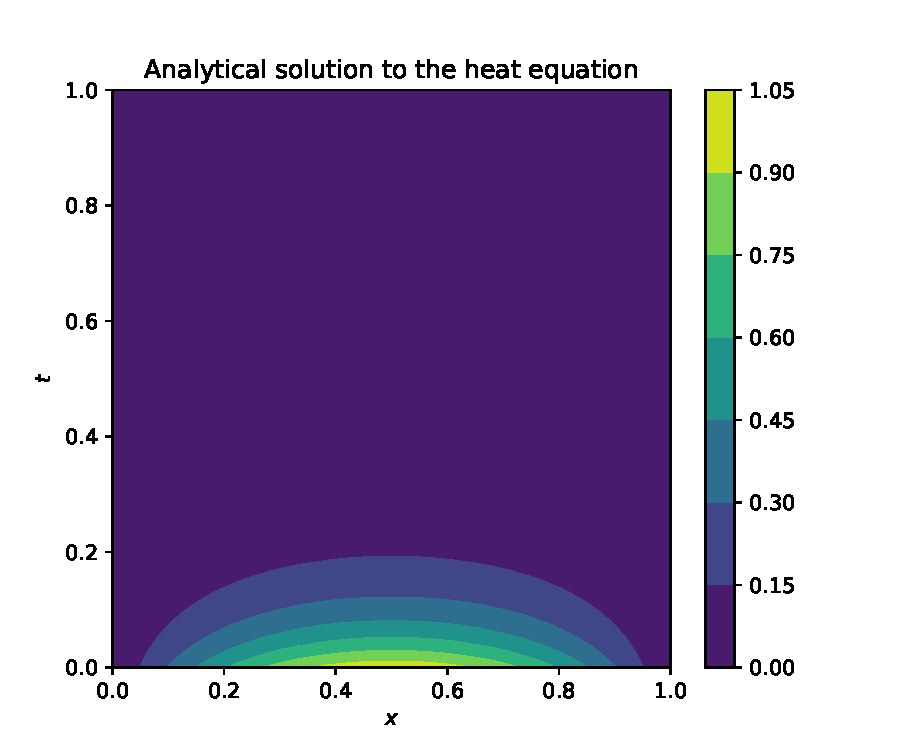
\includegraphics[scale=0.5]{figs/analytical.pdf}
    \caption{Analytical solution to the heat equation.}
    \label{fig:analytical}
\end{figure}

    Having tested our implementations of the finite differences method, neural network and genetic algorithm, we try to evaluate their performance in computing the solution to the heat equation given the boundary conditions described in the beginning of the report. In Figure \ref{fig:analytical}, we can see the analytical solution given by Equation \eqref{eq:heat_anal}, for \(x,t \in [0, 1]^2\).

    For the finite differences method, we run into problems right away. For the stability condition to be satisfied, \(\Delta x\) has to be larger than \(\Delta t\), resulting in a finer resolution in the time domain than in the space domain. This might pose a problem, as when we want to have a higher resolution on the space domain, our time domain will have quadratically more points making the simulation very slow. In Figure \ref{fig:heat_fd}, we see the numerical solution with the finite differences method. We used \(50\) evenly spaced points on the \(x\) axis and \(5000\) evenly spaced points on the \(t\) axis, in order to satisfy the stability condition.

\begin{figure}[htp]
    \centering
    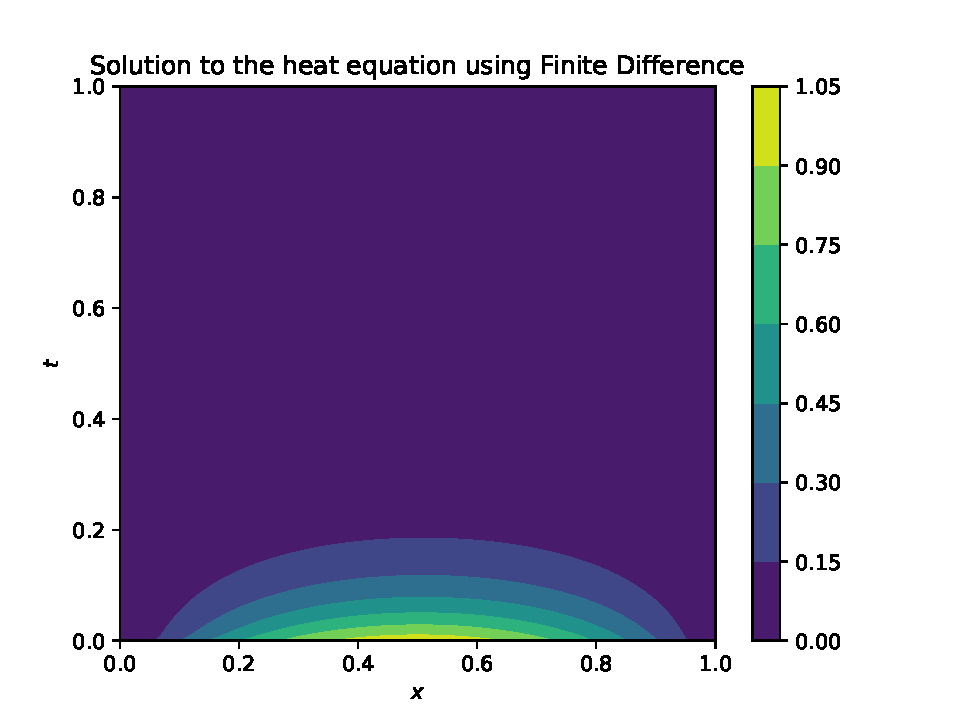
\includegraphics[scale=0.5]{figs/fd/heat_fd_nx_50_nt_5000.pdf}
    \caption{Solution of the heat equation with the finite differences method. Here we used \(50\) points on the \(x\) axis and \(5000\) points on the \(t\) axis. These values were chosen to satisfy the stability condition.}
    \label{fig:heat_fd}
\end{figure}

    As is evident from Figure \ref{fig:error_fd} the finite differences method gives strikingly good results, with the highest absolute error taking place in the beginning region. Exactly why the error appears in the beginning of the calculation is unknown to us, however it was noted that with increased resolution of the \(x\)-axis the error decreased. Due to hardware limitations and the stability requirement, running a highly increased resolution drastically increases computational time, and hence was not performed.

\begin{figure}[htp]
    \centering
    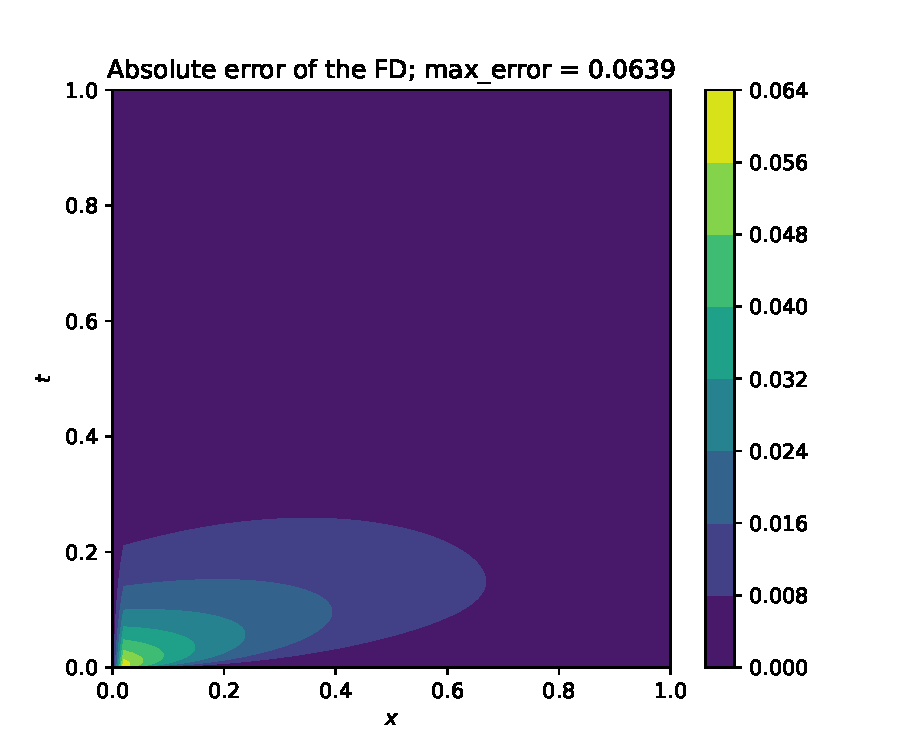
\includegraphics[scale=0.5]{figs/fd/error_fd_nx_50_nt_5000.pdf}
    \caption{Absolute error of the solution of heat equation with the finite differences method against the analytical solution. Here we used \(50\) points on the \(x\) axis and \(5000\) points on the \(t\) axis. These values were chosen to satisfy the stability condition.}
    \label{fig:error_fd}
\end{figure}

    % Gotta add some kind of discussion of the NN results here...
    The neural network finds a solution with a slightly different profile, Figure \ref{fig:heat_nn}. In particular, the temperature at the centre of the rod decays slower in time than found by the analytical solution.
    
    Indeed, the neural network is found to find an absolute error double that of the finite differences method, over a larger region of the domain of interest; especially in \(t \in [0.15, 0.5]\) and \(x \in [0.35, 0.65]\), Figure \ref{fig:error_nn}.

\begin{figure}[htp]
    \centering
    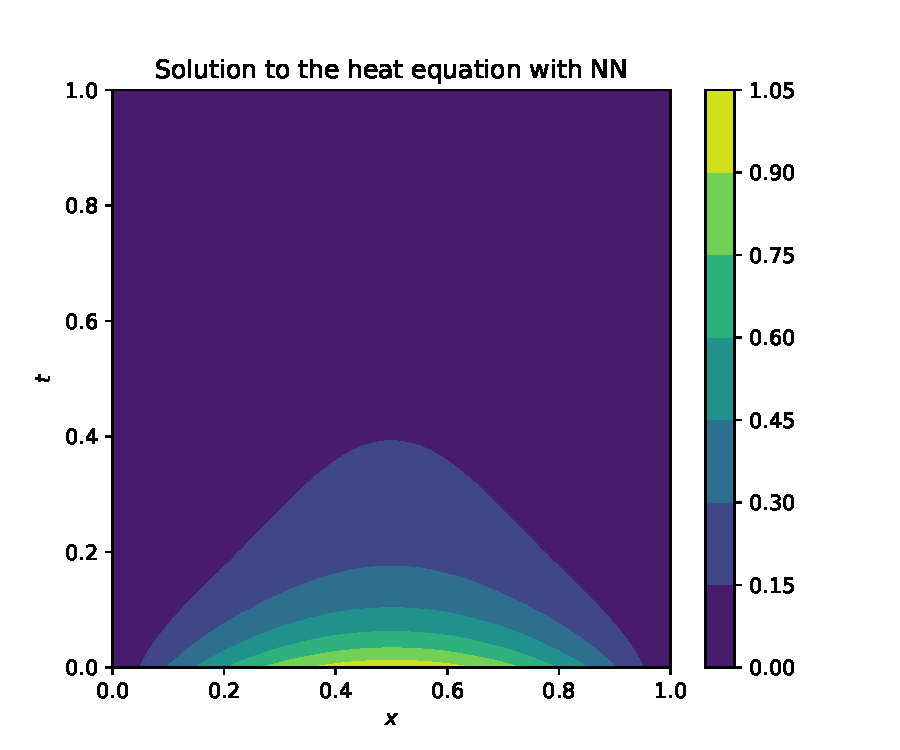
\includegraphics[scale=0.5]{figs/nn/heat_nx_50_nt_50.pdf}
    \caption{Solution of the heat equation with the neural network code. Here we used \(50\) points on the \(x\) axis and \(50\) points on the \(t\) axis. We trained the network for \(5000\) epochs with a learning rate of \(10^{-3}\).}
    \label{fig:heat_nn}
\end{figure}

    That being said, the neural network has the advantage over the finite differences method to be more flexible in how it is setup, in particular in the sample size for discrete points, which makes it a much faster alternative (depending on the grid resolution), at the cost of the lost precision.

\begin{figure}[h]
    \centering
    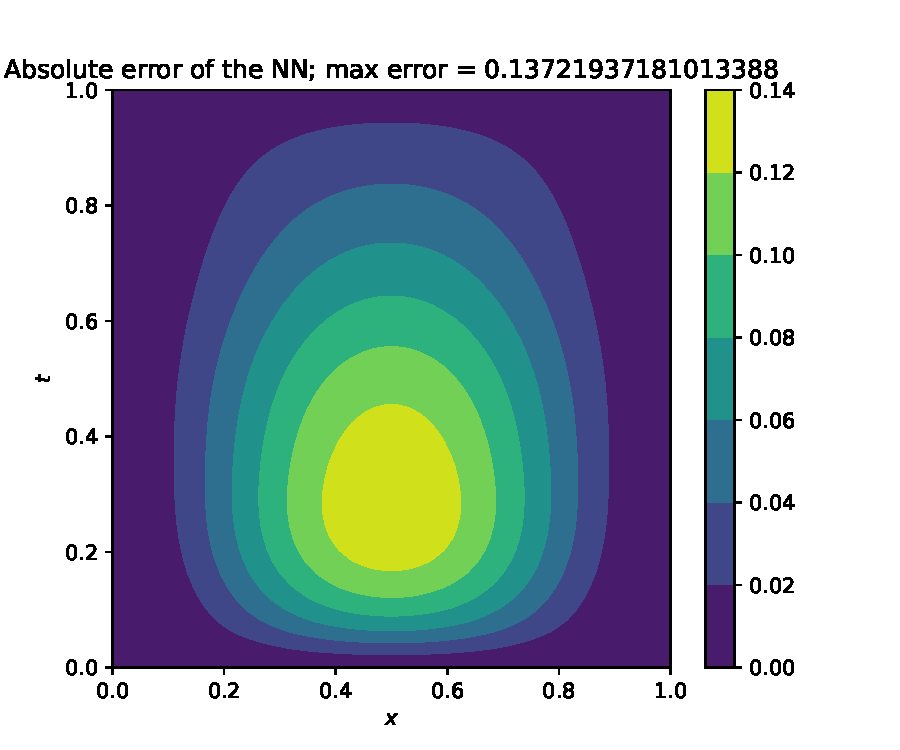
\includegraphics[scale=0.5]{figs/nn/error_nn_nx_50_nt_50.pdf}
    \caption{Absolute error of the solution of heat equation with the neural network code against the analytical solution. Here we used \(50\) points on the \(x\) axis and \(50\) points on the \(t\) axis. We trained the network for \(5000\) epochs with a learning rate of \(10^{-3}\).}
    \label{fig:error_nn}
\end{figure}



% Moved down from the GA section of the results :)
Finally, both genetic methods, as well as the random search, find the solution reliably for the heat equation with \(L = \pi\), putting this PDE on par with PDE4, Figure \ref{fig:generation_counts}. Our method is the only genetic algorithm-based method to find the solution for the heat equation with \(L=1\), around 15\% of the time, in around 4 thousand generations, Figure \ref{fig:generation_counts}; this is likely because of the presence of \(\pi\) in the solution, which is much more difficult to find for the other two methods, which both stall at a fitness value between 100 and 1000, Figure \ref{fig:heat_res}. Our method, when it doesn't find the analytical solution, gets closer than this, with a final fitness of around 10. The two best fits found by the random walk are of the form
    \begin{align*}
        \sigma_{\text{rand}}(x, t) &= \sin(\cos^C(t))
    \end{align*}
    where \(C\) is a very large constant, \(C > 10^5\). The two best fits found by the original method are
    \begin{align*}
        \sigma_{\text{orig}}^{(1)}(x, t) &= 1.04 e^{-7t} \sin(3x)
        \\
        \sigma_{\text{orig}}^{(2)}(x, t) &= \sin(0.63\cos^C(t))
    \end{align*}
    where again \(C\) is a large constant, \(C > 10^8\).
    
    \begin{figure}[htp]
        \centering
        \includegraphics[width=\linewidth]{figs/ga/evolution_comparison_heat.png}
        \caption{Best fitness value at different generations for 10 (randomly selected) individual runs of the three genetic methods, for the heat equation. One run is shown in bold for each of the methods, with 9 other runs displayed in a faded version of the same colour.}
        \label{fig:heat_res}
    \end{figure}
    
    Hence, all three methods we analyse here can be used to solve the heat equation: the finite differences method with a very low error but long computation time; the neural network method with a higher error on average but much quicker to run; and our variation on the grammar-based genetic algorithm method proposed by \cite{solving_diff_reproduce}, which takes a lot longer to run but solves the PDE analytically.

%%%%%%%%%%%%%%%%%%%%%%%%%%%
%%%%%%%%%%%%%%%%%%%%%%%%%%%
\clearpage
\section{Conclusion}
%%%%%%%%%%%%%%%%%%%%%%%%%%%
%%%%%%%%%%%%%%%%%%%%%%%%%%%

The finite differences method was shown to give very precise results and its ability to handle complicated initial and boundary conditions makes it reliable. Unfortunately this is mitigated by the computational load required to make arbitrarily good approximations due to the stability condition. The neural network, however, gives very precise results, in a short amount of time, in the cases where the method is applicable. This unfortunately excludes some of the differential equations in this study, namely ones with Neumann conditions and some PDEs.

As detailed above, the error for the solution given by the genetic algorithm is always 0, as the output \textit{is} the analytical solution. It is also the most flexible of the methods we explored, as it does not impose any limits to the types of functions and boundary conditions that can be represented. However, the genetic algorithm takes much longer to run (up to several hours for non-trivial problems), especially since the success rate increases when initializing several competing populations at once, and so depending on the problem at hand, it may be preferable to fall back on the neural network or finite differences approximation to save time if the approximate solution is good enough in context.

For problems where the closed-form analytical solution is needed (and exists), we recommend using our variation on the original grammar-based genetic algorithm solution proposed by \cite{solving_diff_reproduce} as it converges faster on average for more complicated problems, and has a higher success rate thanks to its greater flexibility. It should be mentioned that we did not focus on optimizing the hyperparameters (reproduction rate, mutation rates, discrete domain sizes and \(\lambda\) penalty), and the genetic operators we implemented were kept fairly simplistic. This entails a sizeable possibility our method could be optimized in order to keep the success rate high but make it converge potentially much faster, either by tweaking the parameters or by implementing a larger collection of genetic operators.

\bibliography{refs.bib}

\onecolumngrid
\appendix
\clearpage

\section{ODEs, NLODEs and PDEs}\label{appendix:ODE_tables}
\begin{table*}[htp]
    \centering
    \caption{The nine ODEs given in the original paper \cite{solving_diff_reproduce}.}
    \begin{tabular}{c|c|l|l|l}
        Label & Domain & ODE & Boundary condition(s) & Solution\\
        \hline
        ODE1 & \([0.1,1]\) & \(\frac{d}{dx}f(x) = \frac{2x-f(x)}{x}\) & \(f(0.1) = 20.1\) & \(f(x) = x + \frac{2}{x}\)
        \\
        ODE2 & \([0.1,1]\) & \(\frac{d}{dx}f(x) = \frac{1-f(x)\cos{(x)}}{\sin{(x)}}\) & \(f(0.1) = \frac{2.1}{\sin{(0.1)}}\) & \(f(x) = \frac{x + 2}{\sin{(x)}}\)
        \\
        ODE3 & \([0,1]\) & \(\frac{d}{dx}f(x) = -\frac{1}{5}f(x) + e^{-x/5}\cos{(x)}\) & \(f(0) = 0\) & \(f(x) = e^{-x/5}\sin{(x)}\)
        \\
        ODE4 & \([0,1]\) & \(\frac{d^2}{dx^2}f(x) = -100 f(x)\) & \(f(0) = 0\), \(\frac{d}{dx}f(0) = 10\) & \(f(x) = \sin{(10 x)}\)
        % \\
        % & & & \(\frac{d}{dx}f(0) = 1\) &
        \\
        ODE5 & \([0,1]\) & \(\frac{d^2}{dx^2}f(x) = 6\frac{d}{dx}f(x) -9 f(x)\) & \(f(0) = 0\), \(\frac{d}{dx}f(0) = 2\) & \(f(x) = 2xe^{3x}\)
        \\
        ODE6 & \([0,2]\) & \(\frac{d^2}{dx^2}f(x) = -\frac{1}{5}\frac{d}{dx}f(x) - f(x) - \frac{1}{5}e^{-x/5}\cos{(x)}\) & \(f(0) = 0\), \(\frac{d}{dx}f(0) = 1\) & \(f(x) = e^{-x/5}\sin{(x)}\)
        \\
        ODE7 & \([0,1]\) & \(\frac{d^2}{dx^2}f(x) = -100 f(x)\) & \(f(0) = 0\), \(f(1) = \sin{(10)}\) & \(f(x) = \sin{(10x)}\)
        \\
        ODE8 & \([0,1]\) & \(x\frac{d^2}{dx^2}f(x) = (x-1) \frac{d}{dx}f(x) - f(x)\) & \(f(0) = 1\), \(f(1) = 0\) & \(f(x) = 1 - x\)
        \\
        ODE9 & \([0,1]\) & \(\frac{d^2}{dx^2}f(x) = -\frac{1}{5}\frac{d}{dx}f(x) - f(x) - \frac{1}{5}e^{-x/5}\cos{(x)}\) & \(f(0) = 0\), \(f(1) = \frac{\sin{(1)}}{e^{0.2}}\) & \(f(x) = e^{-x/5}\sin{(x)}\)
    \end{tabular}
    \label{tab:ODEs}
\end{table*}
\begin{table*}[htp]
    \centering
    \caption{The four non-linear ODEs given in the original paper \cite{solving_diff_reproduce}.}
    \begin{tabular}{c|c|l|l|l}
        Label & Domain & NLODE & Boundary condition(s) & Solution\\
         \hline
        NLODE1 & \([1,4]\) & \(\frac{d}{dx}f(x) = \frac{1}{2f(x)}\) & \(f(1) = 1\) & \(f(x) = \sqrt{x}\)
        \\
        NLODE2 & \([1,2]\) & \(\left(\frac{d^2}{dx^2}f(x)\right)^2 = - \ln{(f(x))} + \cos^2{(x)}\)  & \(f(1) = 1 + \sin{(1)}\) & \(f(x) = x + \sin{(x)}\)
        \\
        & & \qquad\qquad\qquad\(+ 2\cos{(x)} + 1 + \ln{(x+\sin{(x)}})\) & &
        \\
        NLODE3 & \([1,2]\) & \(\left(\frac{d^2}{d^2x}f(x)\right)\frac{d}{dx}f(x) = -\frac{4}{x^3}\) & \(f(1) = 0\) & \(f(x) = \ln{(x^2)}\)
        \\
        NLODE4 & \([e,2e]\) & \(x^2\frac{d^2}{dx^2}f(x) = - \left(x\frac{d}{dx}f(x)\right)^2 - \frac{1}{\ln{(x)}}\) & \(f(e) = 0\), \(\frac{d}{dx}f(e) = e^{-1}\) & \(f(x) = \ln{(\ln{(x)})}\)
    \end{tabular}
    \label{tab:NLODEs}
\end{table*}
\begin{table*}[htp]
    \centering
    % \scalebox{0.7}
    % {
    \caption{Six of the seven PDEs given in the original paper \cite{solving_diff_reproduce}.}
    \begin{tabular}{c|c|l|l|l}
        Label & Domain & PDE & Boundary conditions & Solution\\
        \hline
        PDE1 & \([0,1]^2\) & \(\nabla^2f(x,y) = e^{-x}\left(x-2+y^3+6y\right)\) & \(f(0,y) = y^3\), \(f(1,y) = \left(1+y^3\right)e^{-1}\), & \(f(x,y) = (x + y^3)e^{-x}\)
        \\
        % & & & \(f(x,0) = xe^{-x}\), &
        % \\
        & & & \(f(x,0) = xe^{-x}\), \(f(x,1) = (x+1)e^{-x}\) & \\
        % & & & \(f(0,y) = y^3\) &
        % \\
        PDE2 & \([0,1]^2\) & \(\nabla^2f(x,y) = -2 f(x,y)\) & \(f(0,y) = 0\), \(f(1,y) = \sin(1)\cos(y)\), & \(f(x,y) = \sin{(x)}\cos{(y)}\)
        \\
        % & & & \(f(1,y) = \sin(1)\cos(y)\), &
        % \\
        & & & \(f(x,0) = \sin(x)\), \(f(x,1) = \sin(x)\cos(1)\) &
        \\
        % & & & \(f(x,1) = \sin(x)\cos(y)\) &
        % \\
        PDE3 & \([0,1]^2\) & \(\nabla^2f(x,y) = 4\) & \(f(0,y) = y^2 + y + 1\), \(f(1,y) = y^2 + y + 3\), & \(f(x,y) = x^2+y^2+x+y+1\)
        \\
        % & & & \(f(1,y) = y^2 + y + 3\), &
        % \\
        & & & \(f(x,0) = x^2 + x + 1\), \(f(x,1) = x^2 + x + 3\) &
        \\
        % & & & \(f(x,1) = x^2 + x + 3\) &
        % \\
        PDE4 & \([0,1]^2\) & 
        \(\nabla^2f(x,y) = -\left(x^2+y^2\right)f(x,y)\) & \(f(0,y) = 0\), \(f(1,y) = \sin(y)\), & \(f(x,y) = \sin{(xy)}\)
        \\
        % & & & \(f(1,y) = \sin(y)\), &
        % \\
        & & & \(f(x,0) = 0\), \(f(x,1) = \sin(x)\) &
        \\
        % & & & \(f(x,1) = \sin(x)\) &
        % \\
        PDE5 & \([0,1]^2\) & \(\nabla^2f(x,y) = (x-2)e^{-x} + xe^{-y}\) & \(f(0,y) = 0\), \(f(1,y) = e^{-y} + e^{-1}\), & \(f(x,y) = x(e^{-x} + e^{-y})\)
        \\
        % & & & \(f(1,y) = e^{-y} + e^{-1}\), &
        % \\
        & & & \(f(x,0) = x\left(e^{-x}+1\right)\), \(f(x,1) = x\left(e^{-x}+e^{-1}\right)\) &
        \\
        % & & & \(f(x,1) = x\left(e^{-x}+e^{-1}\right)\) &
        % \\
        PDE6 & \([0,1]^2\) &
        \(\nabla^2f(x,y) + e^{f(x,y)}\) & \(f(0,y) = \ln(1+y^2)\), \(f(1,y) = \ln(2+y^2)\), & \(f(x,y) = \ln(1+x^2+y^2)\)
        \\
        & & \quad\(= 1 + x^2 + y^2 + \frac{4}{\left(1+x^2+y^2\right)^2}\) & \(f(x,0) = \ln(1+x^2)\), \(f(x,1) = \ln(2+x^2)\) &%\(f(1,y) = \ln(2+y^2)\), &
        \\
        % & & & \(f(x,0) = \ln(1+x^2)\), &
        % \\
        % & & & \(f(x,1) = \ln(2+x^2)\) &
    \end{tabular}
    % }
    \label{tab:PDEs}
\end{table*}


\end{document}
% https://tex.stackexchange.com/questions/102546/3d-line-plot-in-pgfplots
% https://no.overleaf.com/learn/latex/Pgfplots_package
% https://tex.stackexchange.com/questions/524337/tikz-pgfplots-plotting-3d-surface-with-cloud-of-points
% https://math.stackexchange.com/questions/404440/what-is-the-equation-for-a-3d-line
% https://www.google.com/search?q=3d+surface+tikz&oq=3d+surface+tik&aqs=chrome.1.69i57j0i22i30l2.6192j0j4&sourceid=chrome&ie=UTF-8
